% Practice Test 16 — Florida Edition
% Questions: 30 (19 MC + 11 SA)
% Generated by scripts/generate_practice_tests.py

\begin{practiceQuestion}{1-3-q24}{sa}
\begin{questionText}
The table shows a proportional relationship. Find $k$ and the missing value.

\begin{center}
\begin{tabular}{|c|c|}
\hline $x$ & $y$ \\ \hline $3$ & $7.5$ \\ $?$ & $15$ \\ $10$ & $25$ \\ \hline
\end{tabular}
\end{center}
\end{questionText}
\correctAnswer{$k = 2.5$; missing $x = 6$}
\explanation{$k = \frac{7.5}{3} = 2.5$. For the missing row: $15 = 2.5x$ so $x = 15 \div 2.5 = 6$.}
\end{practiceQuestion}

\begin{practiceQuestion}{1-6-q27}{gmc}
\begin{questionText}
A map uses the scale shown below. If two cities are $6.5$ cm apart on the map, what is the actual distance?

\begin{center}
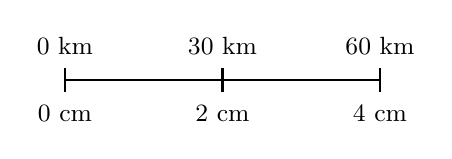
\begin{tikzpicture}[scale=1]
  \draw[thick] (0,0) -- (4,0);
  \draw[thick] (0,-0.15) -- (0,0.15);
  \draw[thick] (2,-0.15) -- (2,0.15);
  \draw[thick] (4,-0.15) -- (4,0.15);
  \node[below] at (0,-0.2) {\small $0$ cm};
  \node[below] at (2,-0.2) {\small $2$ cm};
  \node[below] at (4,-0.2) {\small $4$ cm};
  \node[above] at (0,0.2) {\small $0$ km};
  \node[above] at (2,0.2) {\small $30$ km};
  \node[above] at (4,0.2) {\small $60$ km};
\end{tikzpicture}
\end{center}
\end{questionText}
\choiceA{$90$ km}
\choiceB{$95$ km}
\choiceC{$97.5$ km}
\choiceD{$100$ km}
\correctAnswer{C}
\explanation{Scale: $2$ cm $= 30$ km, so $1$ cm $= 15$ km. For $6.5$ cm: $15 \times 6.5 = 97.5$ km.}
\end{practiceQuestion}

\begin{practiceQuestion}{2-1-q28}{gmc}
\begin{questionText}
The tape diagram below represents a whole quantity. What percent of the total is the shaded portion?

\begin{center}
\begin{tikzpicture}[scale=0.7]
  % Draw 5 equal sections
  \foreach \i in {0,...,4} {
    \draw[thick] (\i*1.6,0) rectangle (\i*1.6+1.6,0.8);
  }
  % Shade 3 of 5 sections
  \fill[funGreen!40] (0,0) rectangle (1.6,0.8);
  \fill[funGreen!40] (1.6,0) rectangle (3.2,0.8);
  \fill[funGreen!40] (3.2,0) rectangle (4.8,0.8);
  \foreach \i in {0,...,4} {
    \draw[thick] (\i*1.6,0) rectangle (\i*1.6+1.6,0.8);
  }
  % Labels
  \node[below,font=\small] at (0.8,0) {$15$};
  \node[below,font=\small] at (2.4,0) {$15$};
  \node[below,font=\small] at (4.0,0) {$15$};
  \node[below,font=\small] at (5.6,0) {$15$};
  \node[below,font=\small] at (7.2,0) {$15$};
  \draw[thick,<->] (0,-0.8) -- (8,-0.8) node[midway,below,font=\small] {Total $= 75$};
\end{tikzpicture}
\end{center}
\end{questionText}
\choiceA{$40\%$}
\choiceB{$45\%$}
\choiceC{$50\%$}
\choiceD{$60\%$}
\correctAnswer{D}
\explanation{The shaded portion is $3 \times 15 = 45$. The total is $75$. Percent: $45 \div 75 = 0.60 = 60\%$.}
\end{practiceQuestion}

\begin{practiceQuestion}{2-2-q07}{mc}
\begin{questionText}
A school has $500$ students. If $68\%$ eat in the cafeteria, how many eat there? Use a proportion.
\end{questionText}
\choiceA{$320$}
\choiceB{$340$}
\choiceC{$350$}
\choiceD{$368$}
\correctAnswer{B}
\explanation{$\frac{n}{500} = \frac{68}{100}$. Cross-multiply: $100n = 34{,}000$. Divide: $n = 340$.}
\end{practiceQuestion}

\begin{practiceQuestion}{2-6-q28}{gmc}
\begin{questionText}
The bar graph shows the interest earned on three different deposits over $2$ years. Which deposit had the highest interest rate?

\begin{center}
\begin{tikzpicture}[scale=0.55]
  \draw[thick,->] (0,0) -- (0,5.5) node[above]{\small Interest (\$)};
  \draw[thick,->] (0,0) -- (7,0);
  \fill[funBlue!60] (0.5,0) rectangle (1.5,2);
  \fill[funGreen!60] (2.5,0) rectangle (3.5,3);
  \fill[funOrange!60] (4.5,0) rectangle (5.5,4);
  \node[below,font=\scriptsize] at (1,0) {$\$500$};
  \node[below,font=\scriptsize] at (3,0) {$\$1{,}000$};
  \node[below,font=\scriptsize] at (5,0) {$\$800$};
  \node[below=12pt,font=\small] at (3,0) {Principal};
  \foreach \y/\lab in {1/25,2/50,3/75,4/100} {
    \draw (-0.1,\y) -- (0.1,\y) node[left,font=\small,xshift=-2pt] {\lab};
  }
  \node[above,font=\small] at (1,2) {$\$50$};
  \node[above,font=\small] at (3,3) {$\$75$};
  \node[above,font=\small] at (5,4) {$\$100$};
\end{tikzpicture}
\end{center}
\end{questionText}
\choiceA{Deposit of $\$500$ (earned $\$50$)}
\choiceB{Deposit of $\$1{,}000$ (earned $\$75$)}
\choiceC{Deposit of $\$800$ (earned $\$100$)}
\choiceD{All have the same rate}
\correctAnswer{C}
\explanation{Rates over $2$ years: $\$500$: $50/(500 \times 2) = 5\%$. $\$1{,}000$: $75/(1{,}000 \times 2) = 3.75\%$. $\$800$: $100/(800 \times 2) = 6.25\%$. The $\$800$ deposit had the highest rate.}
\end{practiceQuestion}

\begin{practiceQuestion}{2-7-q25}{sa}
\begin{questionText}
A jogger estimated running $5$ miles but actually ran $4.8$ miles. What is the percent error (rounded to the nearest tenth)?
\end{questionText}
\correctAnswer{$\approx 4.2\%$}
\explanation{$\frac{|5 - 4.8|}{4.8} \times 100 = \frac{0.2}{4.8} \times 100 \approx 4.17 \approx 4.2\%$.}
\end{practiceQuestion}

\begin{practiceQuestion}{3-2-q27}{gmc}
\begin{questionText}
Which number line correctly models $(-4) + (-3)$?

\begin{center}
\begin{tikzpicture}
  % Model A
  \node[left] at (-7.5,2) {\textbf{A:}};
  \draw[thick,->] (-7,2) -- (3,2);
  \foreach \x in {-6,...,2} \draw (\x,2.1) -- (\x,1.9) node[below] {\footnotesize $\x$};
  \draw[thick,->,funRed] (-4,2.4) -- (-7,2.4);

  % Model B
  \node[left] at (-7.5,0) {\textbf{B:}};
  \draw[thick,->] (-7,0) -- (3,0);
  \foreach \x in {-6,...,2} \draw (\x,0.1) -- (\x,-0.1) node[below] {\footnotesize $\x$};
  \draw[thick,->,funBlue] (-4,0.4) -- (-1,0.4);
\end{tikzpicture}
\end{center}
\end{questionText}
\choiceA{Model A}
\choiceB{Model B}
\choiceC{Both are correct}
\choiceD{Neither is correct}
\correctAnswer{A}
\explanation{$(-4) + (-3)$ means start at $-4$ and move $3$ units left (adding a negative). Model A shows the arrow going from $-4$ to $-7$, which is correct.}
\end{practiceQuestion}

\begin{practiceQuestion}{3-3-q10}{mc}
\begin{questionText}
What is $0 - (-6)$?
\end{questionText}
\choiceA{$-6$}
\choiceB{$6$}
\choiceC{$0$}
\choiceD{$-12$}
\correctAnswer{B}
\explanation{$0 - (-6) = 0 + 6 = 6$. Subtracting a negative is the same as adding.}
\end{practiceQuestion}

\begin{practiceQuestion}{4-4-q22}{sa}
\begin{questionText}
Factor $-8x + 12y - 4$.
\end{questionText}
\correctAnswer{$-4(2x - 3y + 1)$}
\explanation{GCF of $8$, $12$, and $4$ is $4$. Factor out $-4$: $-8x \div (-4) = 2x$, $12y \div (-4) = -3y$, $-4 \div (-4) = 1$. Result: $-4(2x - 3y + 1)$.}
\end{practiceQuestion}

\begin{practiceQuestion}{4-5-q20}{sa}
\begin{questionText}
Simplify $(-3x + 5) + (8x - 12)$.
\end{questionText}
\correctAnswer{$5x - 7$}
\explanation{Combine: $(-3x + 8x) + (5 - 12) = 5x - 7$.}
\end{practiceQuestion}

\begin{practiceQuestion}{5-3-q28}{gmc}
\begin{questionText}
Look at the number line. The expression $3(x + 2)$ equals the distance from $A$ to $B$. What is $x$?

\begin{center}
\begin{tikzpicture}[scale=0.6]
  \draw[thick,->] (-1,0) -- (16,0);
  \foreach \x in {0,3,...,15} \draw (\x,0.15) -- (\x,-0.15) node[below] {$\x$};
  \fill[funBlue] (0,0) circle (4pt) node[above=4pt] {$A$};
  \fill[funOrange] (15,0) circle (4pt) node[above=4pt] {$B$};
  \draw[<->,thick,funBlue] (0,0.6) -- (15,0.6);
  \node[above] at (7.5,0.6) {$3(x+2)$};
\end{tikzpicture}
\end{center}
\end{questionText}
\choiceA{$x = 5$}
\choiceB{$x = 7$}
\choiceC{$x = 3$}
\choiceD{$x = 13$}
\correctAnswer{C}
\explanation{Distance from $A$ to $B$ is $15$. $3(x + 2) = 15$. Divide by $3$: $x + 2 = 5$. Subtract $2$: $x = 3$.}
\end{practiceQuestion}

\begin{practiceQuestion}{5-4-q30}{gsa}
\begin{questionText}
A number line shows a point at $x$. The equation $\dfrac{x}{4} + 1.5 = 5$ tells you how to find $x$. Solve and identify where $x$ is on the number line.

\begin{center}
\begin{tikzpicture}[scale=0.45]
  \draw[thick,->] (-2,0) -- (18,0);
  \foreach \x in {0,2,...,16} {
    \draw (\x,0.2) -- (\x,-0.2) node[below] {$\x$};
  }
  \node[above,funBlue] at (14,0.5) {$x = \;?$};
  \draw[thick,->,funBlue] (14,0.4) -- (14,0.1);
\end{tikzpicture}
\end{center}
\end{questionText}
\correctAnswer{$x = 14$}
\explanation{Subtract $1.5$: $\frac{x}{4} = 3.5$. Multiply by $4$: $x = 14$. The point is at $14$ on the number line.}
\end{practiceQuestion}

\begin{practiceQuestion}{5-5-q23}{sa}
\begin{questionText}
You earn $\$9$ per hour and need more than $\$100$ for a purchase. You already have $\$28$. Write and solve an inequality for the number of hours $h$ you need to work.
\end{questionText}
\correctAnswer{$9h + 28 > 100$; $h > 8$}
\explanation{$9h + 28 > 100$. Subtract $28$: $9h > 72$. Divide by $9$: $h > 8$. You need to work more than $8$ hours.}
\end{practiceQuestion}

\begin{practiceQuestion}{5-6-q01}{mc}
\begin{questionText}
What type of circle is used to graph $x > 3$ on a number line?
\end{questionText}
\choiceA{Closed circle at $3$}
\choiceB{Open circle at $3$}
\choiceC{Closed circle at $0$}
\choiceD{Open circle at $0$}
\correctAnswer{B}
\explanation{$x > 3$ uses an open circle because $3$ is not included (strictly greater than).}
\end{practiceQuestion}

\begin{practiceQuestion}{6-2-q24}{sa}
\begin{questionText}
A drawing uses $1$ cm $= 7$ m. You redraw at $1$ cm $= 7$ m (the same scale). A line is $5$ cm long. How long is it on the new drawing?
\end{questionText}
\correctAnswer{$5$ cm}
\explanation{The scale ratio is $\frac{7}{7} = 1$. The length stays the same: $5 \times 1 = 5$ cm.}
\end{practiceQuestion}

\begin{practiceQuestion}{6-4-q04}{mc}
\begin{questionText}
Two sides of a triangle are $9$ cm and $12$ cm with an included angle of $60°$. What type of condition is this?
\end{questionText}
\choiceA{SSS}
\choiceB{SAS}
\choiceC{ASA}
\choiceD{AAA}
\correctAnswer{B}
\explanation{Two sides and the angle between them is the SAS (Side-Angle-Side) condition.}
\end{practiceQuestion}

\begin{practiceQuestion}{6-5-q22}{sa}
\begin{questionText}
Name two different cross-section shapes you can get from slicing a cube.
\end{questionText}
\correctAnswer{Any two of: square, rectangle, triangle, pentagon, hexagon}
\explanation{A cube can be sliced to produce squares, rectangles, triangles, pentagons, or hexagons depending on the angle and position of the cut.}
\end{practiceQuestion}

\begin{practiceQuestion}{6-6-q21}{sa}
\begin{questionText}
Two vertical angles are $(7x + 1)°$ and $(5x + 13)°$. Find $x$ and the angle measure.
\end{questionText}
\correctAnswer{$x = 6$; the angles are $43°$}
\explanation{Vertical angles are equal: $7x + 1 = 5x + 13$. Subtract $5x$: $2x + 1 = 13$. Subtract $1$: $2x = 12$. Divide: $x = 6$. Angle: $7(6) + 1 = 43°$.}
\end{practiceQuestion}

\begin{practiceQuestion}{7-1-q18}{mc}
\begin{questionText}
A circular garden has a radius of $8$ feet. A path goes straight through the center from one side to the other. How long is the path?
\end{questionText}
\choiceA{$4$ feet}
\choiceB{$8$ feet}
\choiceC{$16$ feet}
\choiceD{$24$ feet}
\correctAnswer{C}
\explanation{The path through the center is a diameter: $d = 2r = 2 \times 8 = 16$ feet.}
\end{practiceQuestion}

\begin{practiceQuestion}{7-5-q18}{mc}
\begin{questionText}
A rectangular prism has a surface area of $94$ cm$^2$. Its length is $5$ cm and width is $3$ cm. What is its height?
\end{questionText}
\choiceA{$2$ cm}
\choiceB{$3$ cm}
\choiceC{$4$ cm}
\choiceD{$5$ cm}
\correctAnswer{C}
\explanation{$94 = 2(5 \times 3) + 2(5 \times h) + 2(3 \times h) = 30 + 10h + 6h = 30 + 16h$. So $16h = 64$, $h = 4$ cm.}
\end{practiceQuestion}

\begin{practiceQuestion}{7-6-q07}{mc}
\begin{questionText}
A cube has a volume of $64$ cm$^3$. What is the side length?
\end{questionText}
\choiceA{$2$ cm}
\choiceB{$4$ cm}
\choiceC{$8$ cm}
\choiceD{$16$ cm}
\correctAnswer{B}
\explanation{$s^3 = 64$. $s = 4$ cm because $4^3 = 64$.}
\end{practiceQuestion}

\begin{practiceQuestion}{7-7-q07}{mc}
\begin{questionText}
A cylinder has a volume of $314$ cm$^3$ and a radius of $5$ cm. What is the height? Use $\pi \approx 3.14$.
\end{questionText}
\choiceA{$2$ cm}
\choiceB{$4$ cm}
\choiceC{$6$ cm}
\choiceD{$10$ cm}
\correctAnswer{B}
\explanation{$V = \pi r^2 h$. $314 = 3.14 \times 25 \times h = 78.5h$. $h = 314 \div 78.5 = 4$ cm.}
\end{practiceQuestion}

\begin{practiceQuestion}{8-1-q04}{mc}
\begin{questionText}
A company wants to know if customers like a new product. They survey only customers who bought the product last week. What is the problem with this sample?
\end{questionText}
\choiceA{The sample is too large}
\choiceB{The sample is biased toward recent buyers}
\choiceC{The sample is random}
\choiceD{There is no problem}
\correctAnswer{B}
\explanation{Only surveying recent buyers introduces bias — they may feel differently than all customers.}
\end{practiceQuestion}

\begin{practiceQuestion}{8-3-q15}{mc}
\begin{questionText}
Group X: mean $45$, range $12$. Group Y: mean $52$, range $12$. What can you say about these groups?
\end{questionText}
\choiceA{They have the same center and different spread}
\choiceB{They have different centers and the same spread}
\choiceC{They are identical}
\choiceD{Group X is more spread out}
\correctAnswer{B}
\explanation{The means differ ($45$ vs.\ $52$) but both have the same range ($12$), so they have different centers and similar spread.}
\end{practiceQuestion}

\begin{practiceQuestion}{8-4-q09}{mc}
\begin{questionText}
The MAD for data set $\{4, 6, 8, 10, 12\}$ with mean $8$ is:
\end{questionText}
\choiceA{$2$}
\choiceB{$2.4$}
\choiceC{$3$}
\choiceD{$8$}
\correctAnswer{B}
\explanation{$|4-8|+|6-8|+|8-8|+|10-8|+|12-8| = 4+2+0+2+4 = 12$. MAD $= \frac{12}{5} = 2.4$.}
\end{practiceQuestion}

\begin{practiceQuestion}{8-5-q28}{gmc}
\begin{questionText}
Use the stem-and-leaf plot to answer the question.

\begin{center}
\begin{tabular}{r|l}
\textbf{Stem} & \textbf{Leaf} \\
\hline
$1$ & $5\;\;8$ \\
$2$ & $0\;\;3\;\;3\;\;7$ \\
$3$ & $1\;\;5\;\;9$ \\
$4$ & $2$
\end{tabular}

Key: $1 \mid 5$ means $15$
\end{center}

How many data values are greater than $25$?
\end{questionText}
\choiceA{$3$}
\choiceB{$4$}
\choiceC{$5$}
\choiceD{$6$}
\correctAnswer{C}
\explanation{Values greater than $25$: $27, 31, 35, 39, 42$ — that's $5$ values.}
\end{practiceQuestion}

\begin{practiceQuestion}{8-6-q10}{mc}
\begin{questionText}
A class of $40$ students: $16$ prefer dogs, $12$ prefer cats, $8$ prefer fish, $4$ prefer birds. What percent prefer dogs?
\end{questionText}
\choiceA{$16\%$}
\choiceB{$25\%$}
\choiceC{$40\%$}
\choiceD{$80\%$}
\correctAnswer{C}
\explanation{$\frac{16}{40} = 0.40 = 40\%$.}
\end{practiceQuestion}

\begin{practiceQuestion}{9-4-q20}{sa}
\begin{questionText}
A probability model has outcomes X, Y, and Z. $P(X) = 0.15$ and $P(Y) = 0.45$. What is $P(Z)$?
\end{questionText}
\correctAnswer{$0.4$}
\explanation{$P(Z) = 1 - 0.15 - 0.45 = 0.40$.}
\end{practiceQuestion}

\begin{practiceQuestion}{9-6-q12}{mc}
\begin{questionText}
A spinner has $4$ equal sections ($1, 2, 3, 4$) and a die is rolled. What is the probability that both show a $3$?
\end{questionText}
\choiceA{$\frac{1}{10}$}
\choiceB{$\frac{1}{24}$}
\choiceC{$\frac{2}{10}$}
\choiceD{$\frac{1}{4}$}
\correctAnswer{B}
\explanation{$P(\text{spinner} = 3) = \frac{1}{4}$, $P(\text{die} = 3) = \frac{1}{6}$. $P = \frac{1}{4} \times \frac{1}{6} = \frac{1}{24}$.}
\end{practiceQuestion}

\begin{practiceQuestion}{9-7-q23}{sa}
\begin{questionText}
A spinner has a $60\%$ chance of landing on blue. In a simulation of $80$ spins, how many times would you expect blue to appear?
\end{questionText}
\correctAnswer{$48$}
\explanation{$80 \times 0.60 = 48$.}
\end{practiceQuestion}
